\documentclass[11pt]{article} 
% ~~~~~~~~~~~~~~~~~~~~~~~~~~~~~~~~~~~~~~~~~~~~~~~~~~~~~ %
\input{./Scripts/packages}	
\input{./Scripts/ridefinitions}
\input{./Scripts/figuresgraphicalsettings}
\input{./Scripts/tablesgraphicalsettings}
\input{./Scripts/newcommands}
% Definition of blocks:
\tikzset{%
  block/.style    = {draw, thick, rectangle, minimum height = 3em,
    minimum width = 3em},
  sum/.style      = {draw, circle, node distance = 2cm}, % Adder
  input/.style    = {coordinate}, % Input
  output/.style   = {coordinate} % Output
}
% Defining string as labels of certain blocks.
\newcommand{\suma}{\Large$+$}
\newcommand{\inte}{$\displaystyle \int$}
\newcommand{\derv}{\huge$\frac{d}{dt}$}
% ~~~~~~~~~~~~~~~~~~~~~~~~~~~~~~~~~~~~~~~~~~~~~~~~~~~~~ %

\title{\Huge ELEC-E8101 Group project: \\ Lab B report \\ Group 11}
\date{\today}
\author{HOUILLE Florent, MONTE SASTRE Enrique, SOULARD Yoann, WANG Tong}


\begin{document}
\maketitle

%/////////////////////////////////////////////////////////////%
%/////////////////////////TASK 5.1/////////////////////////%
%/////////////////////////////////////////////////////////////%
\subsection*{Reporting of Task 5.1}

We implemented our PID with the values we obtained in lab A. Unfortunately, the sampling time (42ms) was not working at all. The robot's wheels were just stuck, making a nearly imperciptible back and forth movement. If the sampling time would have been too high, the system would have been unstable and the command would have maxed the limit out right at the beginning. So we didn't find a good reason to explain this behaviour. We tried to bend the robot to force the wheels in one particular direction, but still they are alterning quickly between forward and backward movement.
So instead we used the minimum sampling time (5 ms) and tuned the PID's parameter to finally obtain :

\begin{equation*}
K_p=-250   ;   K_i=-500   ;   K_d=-0.6
\end{equation*}

Actually these parameters were difficult to tune because the robot's behaviour is highly depend of its initial angle. For instance sometimes it could stay up for more than 5 seconds and other times it fell in only 1 second with the exact same parameters set. We decreased $K_p$ to get a smoother behaviour around the null angle (i.e. improve stability, prevent jitters). We decreased integral term to prevent overshoot (once the robot reached the null angle, it was falling the other side). We increased derivative term so that the robot is better ``aware'' that it is going to fall down and can act before it's too late. Here is a result we recorded with Simulink :

\begin{figure}[H]
\centering
\subfloat[$u(t)$]{
  	\includegraphics[width=\linewidth/2]{LabB/Task51_u.pdf}
  }
  \\
  \subfloat[$\theta_b(t)$]{
  	\includegraphics[width=\linewidth/2]{LabB/Task51_thetab.pdf}
  }
   \subfloat[$x_w(t)$]{
  	\includegraphics[width=\linewidth/2]{LabB/Task51_xw.pdf}
  }
  \caption{Simulation results (the robot falls after 5.5 seconds)}
  \label{fig:fig1}
\end{figure}

The command goes at its maximum value at $t=5 s$. It corresponds to the time when the robot stops moving (i.e. $x_w$ is stabilized), before going the other way. We think this brutal command is the reason why the robot fell down.
One can also notice that the command is oscillating. This might be due to high frequency noises coming from the sensors and then transmitted to the PID's derivative action (we didn't use any filter).

%/////////////////////////////////////////////////////////////%
%/////////////////////////TASK 5.2/////////////////////////%
%/////////////////////////////////////////////////////////////%
\subsection*{Reporting of Task 5.2}

%/////5.2.1/////%
5.2.1 Here are the controllability $\mathcal{C}$ and observability $\mathcal{O}$ matrices in parametric and numeric form (according to lab A state-space):

\begin{equation*}
\mathcal{C}=
	\begin{bmatrix}
	B & AB & AAB
	\end{bmatrix}
	=1.10^5
	\begin{bmatrix}
	0 & 0 & 4.10^{-4} & \approx0 \\
	4.10^{-4} & \approx0 & -0.3087 & -1.44.10^{-2} \\
	0 & 0 & -1.6.10^{-3} & \approx0 \\
	-1.6.10^{-3} & \approx0 & 1.3216 & 6.15.10^{-2}
	\end{bmatrix}
\end{equation*}
\begin{equation*}
\mathcal{O}=
	\begin{bmatrix}
	C \\
	AC \\
	AAC \\
	AAAC \\
	\end{bmatrix}
	=1.10^6
	\begin{bmatrix}
	0 & 0 & \approx0 & 0 \\
	0 & 0 & 0 & \approx0 \\
	0 & 3.3.10^{-3} & 1.10^{-4} & -1.10^{-4} \\
	0 & -2.7943 & -0.0262 & 0.0587
	\end{bmatrix}
\end{equation*}
\begin{equation*}
\Delta\mathcal{C}=-1.10^{-5} \;\; \Delta\mathcal{O}=0
\end{equation*}

$\mathcal{C}$ matrice is full-rank (4), therefore the system is controllable. 
$\mathcal{O}$ matrice is not full-rank, therefore the system is non-observable.


%/////5.2.2.a/////%
5.2.2 a) Our system is non-observable. The system is unobservable if there is at least one state we can’t observe. When we represented the system state space form, C matrix had 3 null columns (out of 4). That’s why our system is unobservable.
This can be due to some missing physical sensors.\\

%/////5.2.2.b/////%
5.2.2 b) In order to have an observable system, we just need to make the component $x_w$ observable. Once $x_w$ and $\theta_b$ are observable, we can then derive other states $\dot x_w$ and $\dot \theta_b$. We can not add a sensor to physcally measure $x_w$ but one can get it from the wheels' angular speed and diameter.\\

%/////5.2.2.c/////%
5.2.2 c) We just added a component to C, therefore we will have two outputs :

\begin{equation*}
C=
\begin{bmatrix}
1 & 0 & 0 & 0\\
0 & 0 & 1 & 0\\
\end{bmatrix}
\end{equation*}


%/////////////////////////////////////////////////////////////%
%/////////////////////////TASK 5.3/////////////////////////%
%/////////////////////////////////////////////////////////////%
\subsection*{Reporting of Task 5.3}

%/////5.3.1/////%
5.3.1 Here are the eigen values of the matrix A before any modification (some are approximated) :
\begin{equation*}
p_1=0 \qquad p_2=-843.4 \qquad p_3=-5.6 \qquad p_4=5.7
\end{equation*}

One can see that one pole is an integrator ($p_1=0$), another is unstable ($p_4>0$), another is stable but slow ($p_3$) and the last is stable and fast, we can keep it as is ($p_2$).
First, we want all the poles to be stable ($<0$).Then, we want to approximate the system as being second order. Therefore, we can choose two dominant poles such that two other poles can be negligated. One can say that a ratio of 6 is enough to declare a pole as negligeable. Therefore, we can take :
\begin{equation*}
p_1=-2 \qquad p_2=-843.4 \qquad p_3=-12 \qquad p_4=-3
\end{equation*}
The ratio between poles is the only thing that matters, but we also took poles with small magnitude in order to have a realistic controller (i.e. $p_1$ and $p_4$ are slow enough so that they won't require the controller to provide too much energy).
So now $p_2$ and $p_3$ can be negligated compared to the slowest pole $p_1$. We end up with the following poles:
\begin{equation*}
p_1=-2 \qquad p_2=-3
\end{equation*}

%/////5.3.2/////%
5.3.2 We want to find a gain matrix $K$ such that eigen values of $A-BK$ are equals to the poles previsouly chosen. For that, one can use the Matlab function \emph{place} to which we provide mtrices $A$,$B$ and the chosen poles vector. We obtain the following values:
\begin{equation*}
K=
\begin{bmatrix}
-47.5 & -64.7 & -103.4 & -15.2
\end{bmatrix}
\end{equation*}

%/////5.3.3/////%
5.3.3 We then implement this SS controller in Simulink and obtain the following result:
\begin{figure}[H]
\subfloat[$u(t)$]{
  	\includegraphics[width=\linewidth]{LabB/Task53_ssCtrl_vm.pdf}
  }
  \\
  \subfloat[$\theta_b(t)$]{
  	\includegraphics[width=\linewidth]{LabB/Task53_ssCtrl_Thetab.pdf}
  }
  \caption{Simulation results with first SS controller}
  \label{fig:fig2}
\end{figure}
One can notice that the system is stable (the robot doesn't fall). Moreover, the command is realistic as the voltage does not go beyond 6 Volts (batteries full capacity is 7.2V).


%/////////////////////////////////////////////////////////////%
%/////////////////////////TASK 5.4/////////////////////////%
%/////////////////////////////////////////////////////////////%
\subsection*{Reporting of Task 5.4}
Unfortunately, we were not able to compute the reduced order estimator.
The reason is that we found some problems following the guide with the notations, so finally when trying to compute $M_1$, $M_2$ etc, it was not possible because of matrix dimension problems in multiplications.
However, the code of what we tried is attached.
First thing we did is to select a $V$ such that the $z$ obtained is an identity matrix. $V$ should be a 3x4 matrix in order to have an invertible T. Therefore :
\begin{equation*}
V=
\begin{bmatrix}
0 & 1 & 0 & 0 \\
0 & 0 & 1 & 0 \\
0 & 0 & 0 & 1
\end{bmatrix}
\end{equation*}

Therefore, future calculations will be easier with $z$ as an identity matrix.

Later, we just tried to follow the steps (and understand them) in the guideline and when we reached the $M_1$ parameter calculation it was not possible to compute it because of matrix dimension error in multiplication. We suspect the problem to be a wrong choice in our matrices but we tried to read again and again the guideline and despite this we lost ourselves in the variables notations.



%/////////////////////////////////////////////////////////////%
%/////////////////////////TASK 5.5/////////////////////////%
%/////////////////////////////////////////////////////////////%
\subsection*{Reporting of Task 5.5}
%/////5.5.1/////%
5.5.1 We formed a state-space system with the matrices $A$,$B$,$C$ and $D$. Then we discretized this ss into a discrete one with a sampling time of $h=5 ms$ and the zero-holder method using Matlab's c2d function.

5.5.2 Then we map all poles chosen previously from $s$- to $z$-domain applying the equivalence formula $z_i=e^{p_ih}$.


\subsection*{Lab B conclusion}
During this lab we tested our Lab A's PID on the robot and obtained quite good result for this kind of controller. We tried to improve it before designing a more advanced state-space controller by pole placement method. It worked on simulation but we didn't try it on the robot. Then we tried to design a state observer. We obtained the full order one, but unfortunately didn't manage to compute the reduced order one. We should work deeper on this topic for the exam...
A lack of time prevented us from doing some simulations and tests over the robot.

\end{document}

%	INLINE EQUATION FORMAT
% This is an example sentence with this formula : $x=50$

%	BOLD TEXT
%\textbf{Type text here}

%	FRACTION
%\frac{Numerator}{Denominator}

%	 MATRIX with brackets like this : [ ]
%\begin{equation*}
%x=
%	\begin{bmatrix}
%	x_11 & x_12\\
%	x_21 & x_22\\
%	x_31 & x_32\\
%	\end{bmatrix}
%\end{equation*}

%	SYSTEM OF EQUATIONS
%\begin{align*}
%\begin{cases}
% equation1 left part = equation1 right part\\
% equation2 left part = equation2 right part\\
%\end{cases}
%\end{align*}

%	1 FIGURE centered just after the text, with a description and a number
%\begin{figure}[H]
%  \includegraphics[width=\linewidth]{LabFolder/ImageName.png}
%  \caption{Description of figure}
%  \label{fig:fig1}
%\end{figure}

%	4 FIGURES displayed 2 by 2 , with a global description
%\begin{figure}[H]
%  \includegraphics[width=\linewidth/2]{LabA/Task45_xw.pdf}
%  \includegraphics[width=\linewidth/2]{LabA/Task45_Thetaw.pdf}
%  \includegraphics[width=\linewidth/2]{LabA/Task45_vw.pdf}
%  \includegraphics[width=\linewidth/2]{LabA/Task45_d.pdf}
%  \caption{Simulation results}
%  \label{fig:fig4}
%\end{figure}

%	4 FIGURES displayed 2 by 2 , with a description for each
%\begin{figure}[H]
%\begin{subfigure}[b]{0.5\linewidth}
%  \includegraphics[width=\linewidth]{LabA/Task48_vmDiscXTraMass0kg500g.pdf}
%  \caption{description 1}
%\end{subfigure}
%\begin{subfigure}[b]{0.5\linewidth}
%  \includegraphics[width=\linewidth]{LabA/Task48_vmDiscXTraMass1kg.pdf}
%    \caption{description 2}
%\end{subfigure}
%\begin{subfigure}[b]{0.5\linewidth}
%  \includegraphics[width=\linewidth]{LabA/Task48_vmDiscXTraMass3kg.pdf}
%    \caption{description 3}
%\end{subfigure}
%\begin{subfigure}[b]{0.5\linewidth}
%  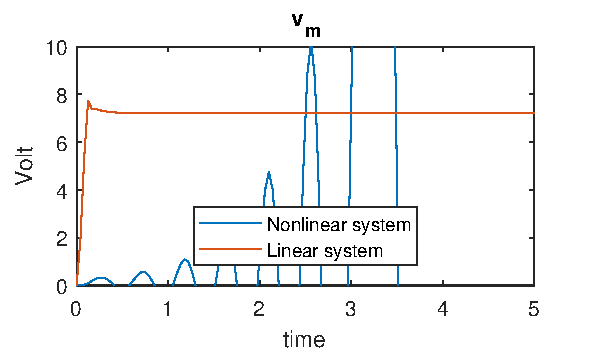
\includegraphics[width=\linewidth]{LabA/Task48_vmDiscXTraMass25kg.pdf}
%    \caption{description 4}
%\end{subfigure}
%  \caption{General description}
%  \label{fig:fig7}
%\end{figure}
